The code for \Fflip is quite simple and shown below:
\begin{lstlisting}[basicstyle=\scriptsize\BeraMonottFamily, frame=single, mathescape]
$\nproc$ F_coinflip[K]{p2fn}{m} :
  (k: Int), (rng: [Bit]), (sid: session[1]),
  ($\$$F: flipper[$\tp{K}$]{$\tp{p2fn}$}{$\tp{f2pn}$}), ($\$$R: receiver[$\tp{K}$]{$\tp{p2fn}$}{$\tp{f2pn}$}),
  ($\$$A: adv[$\tp{K}$]) |- ($\$$c: 1) =
{
  $\ncase$ $\$$F (
    init =>
      x = $\nrecv$ $\$$F ;
      $\nget$ $\$$F {p2fn}
      b = sample 1 rng ;
      $\$$A.flipped ;
      $\nsend$ $\$$A x ;
      $\tg{(* wait for getflips *)}$
      $\$$f <- getflip_f{$\tp{p2fn}$}{$\tp{f2pn}$} <- b $\$$F ;
      $\$$r <- getflip_r[$\tp{K}$]{$\tp{p2fn}$}{$\tp{f2pn}$} <- b x $\$$R ;
  )
}
\end{lstlisting}
We elide the code for \inline{getflip} although it is straightforward. 
The adversary decides whether to deliver the output flip to a party asking for it.
Much like the real-world case where the corrupt committer never opens its commitment, the simulator here can ensure that only the flipper receives the flip.
As the session type indicates, the adversary responds with a \inline{yes} or \inline{no} to deliver the flip.

\subsection{Simulator}
The protocol for the coin flip uses \Fcom. 
The flipper commits to a bit $b$, the receiver sends the flipper a random bit $r$ in return, the flipper opens its commitment, and both parties compute the flip as $r \oplus b$.
The simulator for this protocol to realize \Fflip is straightforward:
\begin{itemize}
\item If the flipper is corrupt, the simulator tells the flipper to \inline{init} the flip when the environment sends it a \inline{Commit b} message. It gets the flip outcome $f$ from the flipper and simulates the receivers random bit $r = f \oplus b$ for the environment. It never delivers the flip outcome to the receiver unless the environment instructs it to open the flipper's commitment. By setting $r = f \oplus b$, when the environment receives $f$ it can check that $r \oplus b = f$.
\item If the receiver is corrupt, the simulator waits for \Fflip to inform it that the flip was initiated. It simulates the \inline{Commit} message from \Fcom to the receiver, for \Z. When it receives the random bit that \Z wants the receiver to send, it gets the flip outcome from the receiver, computes $b = r \oplus f$ and sends \inline{Open b} to \Z. Again, \Z can verify $b \oplus r$ similar to the above case.
nl
\end{itemize}

\subsection{Composition}
We describe a composition theorem in the previous section, a composition operator for protocols, and a brief highlight of the composition operator for simulators.
Composition of the coin flip with the commitment protocol is realized with simulator composition in exactly this way.
We give a diagram of simulator composition in~\ref{fig:simcomp}.
\begin{figure}
\centering
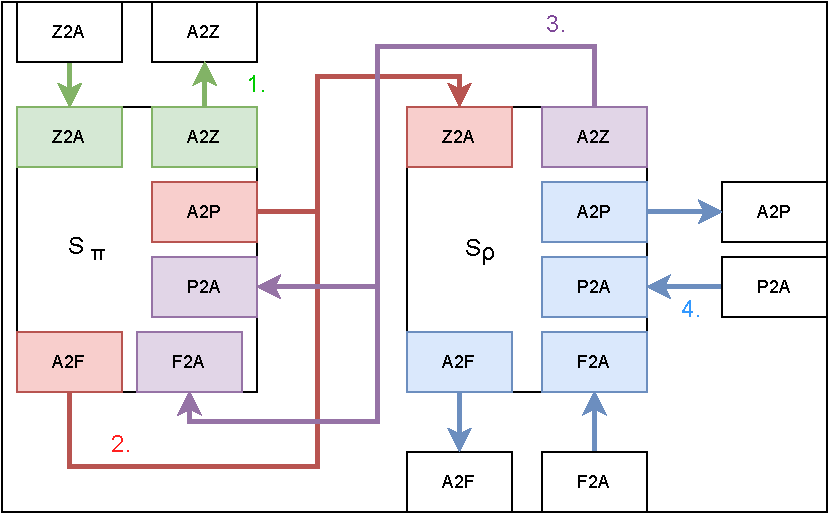
\includegraphics[scale=0.5]{figures/simcomp.pdf}
\caption{The composed simulators for $\F_1 \xrightarrow{\rho \circ \pi} \F_3$. The real world consists of $(\rho \circ \pi, \F_1)$. Inputs from \Z are for $\F_1$ and dummy parties interacting with $\F_1$, which \SIM{\pi} is equipped to handle. Outputs from \SIM{\pi} are for $\F_2$ and dummy parties of $\F_2$ which \SIM{\rho} is equipped to handle. Finally, outputs from \SIM{\rho} are for $\F_3$ and dummy parties of $\F_3$, which is just the ideal world in Theorem~\ref{thm:composition}.}
\label{fig:simcomp}
\end{figure}
